\documentclass[12pt]{article}
\usepackage{amsmath}
\usepackage{graphicx}
\usepackage{hyperref}
\usepackage{ctex}
\usepackage{float}
\usepackage{longtable}
\title{LAB1实验报告}
\author{罗庵瑞 PB24511942}
\date{\today}

\begin{document}

\maketitle

\section{实验背景与目标}


本实验旨在通过补全线性回归和逻辑回归模型的代码,深入理解模型的构建与训练过程。实验的主要任务是实现数据预处理、模型训练以及回归方法的应用。实验的目标是通过调整模型参数与数据预处理策略,观察模型在训练集和验证集上的表现。

\section{实验过程}

\subsection{数据集预处理}
本实验使用的数据集主要是GPU在不同任务中的表现。我对数据集进行了标准化处理,以确保各特征在同一尺度上进行比较。具体的预处理步骤包括:
\begin{itemize}
    \item \textbf{数据提取:} 从原始数据集中提取相关features和targets,并将其存储为NumPy数组,方便后续处理。
    \item \textbf{标准化:} 对features进行标准化处理,使其均值为0,标准差为1,以提高模型训练的稳定性和收敛速度。
\end{itemize}

\subsection{完成模型}

本实验实现了两种经典的回归模型:线性回归和逻辑回归,分别用于回归任务和二分类任务。以下是对每个模型的详细介绍。

\subsubsection{线性回归模型}

线性回归模型用于预测连续值输出。该模型通过最小化均方误差损失函数来拟合输入特征与目标之间的关系。模型的核心部分如下:

\begin{itemize}
    \item \textbf{初始化:} 在模型初始化时,weight通过随机初始化,bias初始化为零。
    \item \textbf{前向传播:} 使用输入特征计算预测结果,公式为:
    \[
    \hat{y} = X \cdot W + b
    \]
    其中,$X$ 为输入特征矩阵,$W$ 为权重,$b$ 为偏置。
    \item \textbf{梯度计算:} 使用MSE损失函数计算梯度。梯度用于更新模型参数,以最小化损失函数。损失函数为:
    \[
    \text{MSE} = \frac{1}{N} \sum_{i=1}^{N} (y_i - \hat{y}_i)^2
    \]
    其中,$y_i$ 是真实值,$\hat{y}_i$ 是预测值。
    \item \textbf{反向传播:} 通过计算梯度并使用学习率对权重和偏置进行更新,更新规则为:
    \[
    W \leftarrow W - \eta \cdot \nabla_W \quad \text{和} \quad b \leftarrow b - \eta \cdot \nabla_b
    \]
    其中,$\eta$ 为学习率,$\nabla_W$ 和 $\nabla_b$ 分别为对权重和偏置的梯度。
\end{itemize}
\subsubsection{线性回归的解析解}

线性回归有解析解,可以通过最小二乘法直接求解权重和偏置。解析解的计算公式如下:
\[
\theta = (X^T X)^{-1} X^T y
\]
其中,$X$ 是输入特征矩阵,$y$ 是真实值,$\theta$ 是包含权重和偏置的参数向量。通过对比模型的结果和解析解的结果,可以判断模型的性能。

\subsubsection{逻辑回归模型}

逻辑回归模型用于二分类任务,输出值为类别的概率。该模型采用 sigmoid 函数将线性组合的结果映射到0到1之间的概率值。具体实现如下:

\begin{itemize}
    \item \textbf{初始化:} 与线性回归类似,权重和偏置也通过随机初始化,偏置初始化为零。
    \item \textbf{前向传播:} 通过计算线性组合并应用 sigmoid 激活函数得到输出概率:
    \[
    p = \sigma(X \cdot W + b) = \frac{1}{1 + e^{-(X \cdot W + b)}}
    \]
    其中,$\sigma$ 是 sigmoid 函数,$X$ 是输入特征,$W$ 是权重,$b$ 是偏置。
    \item \textbf{梯度计算:} 使用binary cross-entropy计算损失并求梯度,损失函数定义为:
    \[
    \text{Loss} = -\frac{1}{N} \sum_{i=1}^{N} \left[ y_i \log(p_i) + (1 - y_i) \log(1 - p_i) \right]
    \]
    其中,$y_i$ 是实际标签,$p_i$ 是预测的概率。
    \item \textbf{反向传播:} 计算对权重和偏置的梯度,更新规则为:
    \[
    W \leftarrow W - \eta \cdot \nabla_W \quad \text{和} \quad b \leftarrow b - \eta \cdot \nabla_b
    \]
    其中,$\nabla_W$ 和 $\nabla_b$ 分别是权重和偏置的梯度,$\eta$ 为学习率。
\end{itemize}

\subsection{模型训练}

为了训练上述模型,我们设计LinearRegressionTrainer和LogisticRegressionTrainer类,分别用于线性回归和逻辑回归的训练。每个训练类都继承自Trainer类,并实现了以下功能:

\begin{itemize}
    \item \textbf{损失计算:} 通过调用模型的 \texttt{compute\_loss} 方法,计算每个批次的loss。
    \item \textbf{梯度更新:} 通过反向传播计算梯度并更新模型参数,使用批量梯度下降优化参数。
    \item \textbf{评估:} 每个训练周期结束后,进行模型评估。
\end{itemize}

\subsection{模型评估与分析}

在训练过程中分别训练集和验证集上评估模型性能。通过观察损失函数值的变化判断模型是否收敛,并以此调整超参数,以提高模型的准确性和泛化能力,寻找最优结果。


\section{调整超参数}

\subsection{超参数选择与调整}
主要调整了Batch Size,Learning Rate,Epochs三个超参数,分别取128,256,512;1e-4,1e-3,1e-2;10,50,100,记录结果并得到表格,从表格来看超参数的调整范围涵盖了最好结果  

\subsection{调整结果}
\begin{table}[htbp]
\centering
\caption{不同超参数下的线性回归模型性能比较}
\begin{tabular}{cccccc}
\hline
\textbf{Batch Size} & \textbf{Learning Rate} & \textbf{Epochs} & \textbf{Train Time (s)} & \textbf{MAE} & \textbf{$R^2$} \\
\hline
128 & 0.0001 & 10 & 7.84 & 0.55 & 0.42 \\
128 & 0.0001 & 50 & 5.51 & 0.55 & 0.42 \\
128 & 0.0001 & 100 & 10.07 & 0.55 & 0.42 \\
128 & 0.001 & 10 & 2.30 & 0.55 & 0.42 \\
128 & 0.001 & 50 & 5.75 & 0.55 & 0.42 \\
128 & 0.001 & 100 & 12.79 & 0.55 & 0.42 \\
128 & 0.01 & 10 & 5.55 & 0.55 & 0.42 \\
128 & 0.01 & 50 & 14.48 & 0.55 & 0.42 \\
128 & 0.01 & 100 & 9.66 & 0.55 & 0.42 \\
256 & 0.0001 & 10 & 1.89 & 0.55 & 0.42 \\
256 & 0.0001 & 50 & 3.68 & 0.55 & 0.42 \\
256 & 0.0001 & 100 & 5.97 & 0.55 & 0.42 \\
256 & 0.001 & 10 & 1.88 & 0.55 & 0.42 \\
256 & 0.001 & 50 & 3.74 & 0.55 & 0.42 \\
256 & 0.001 & 100 & 5.93 & 0.55 & 0.42 \\
256 & 0.01 & 10 & 1.95 & 0.55 & 0.42 \\
256 & 0.01 & 50 & 3.79 & 0.55 & 0.42 \\
256 & 0.01 & 100 & 6.05 & 0.55 & 0.42 \\
512 & 0.0001 & 10 & 1.74 & 0.55 & 0.42 \\
512 & 0.0001 & 50 & 2.84 & 0.55 & 0.42 \\
512 & 0.0001 & 100 & 4.21 & 0.55 & 0.42 \\
512 & 0.001 & 10 & 1.76 & 0.55 & 0.42 \\
512 & 0.001 & 50 & 2.82 & 0.55 & 0.42 \\
512 & 0.001 & 100 & 4.17 & 0.55 & 0.42 \\ 
512 & 0.01 & 10 & 1.76 & 0.55 & 0.42 \\
512 & 0.01 & 50 & 2.83 & 0.55 & 0.42 \\
512 & 0.01 & 100 & 4.16 & 0.55 & 0.42 \\
\hline
\end{tabular}
\label{tab:regression_results}
\end{table}

\begin{table}[htbp]
\centering
\caption{不同超参数下的分类模型性能比较}
\begin{tabular}{ccccccc}
\hline
\textbf{Batch Size} & \textbf{Learning Rate} & \textbf{Epochs} & \textbf{Train Time (s)} & \textbf{F1} & \textbf{AUC} \\
\hline
128 & 0.0001 & 10 & 2.56 & 0.67 & 0.74 \\
128 & 0.0001 & 50 & 6.87 & 0.72 & 0.78 \\
128 & 0.0001 & 100 & 12.23 & 0.75 & 0.80 \\
128 & 0.001 & 10 & 2.55 & 0.75 & 0.80 \\
128 & 0.001 & 50 & 6.95 & 0.79 & 0.83 \\
128 & 0.001 & 100 & 12.32 & 0.79 & 0.83 \\
128 & 0.01 & 10 & 2.58 & 0.79 & 0.83 \\
128 & 0.01 & 50 & 7.15 & 0.79 & 0.83 \\
128 & 0.01 & 100 & 12.43 & 0.79 & 0.83 \\
256 & 0.0001 & 10 & 2.08 & 0.65 & 0.72 \\
256 & 0.0001 & 50 & 4.38 & 0.70 & 0.76 \\
256 & 0.0001 & 100 & 7.29 & 0.72 & 0.78 \\
256 & 0.001 & 10 & 2.09 & 0.72 & 0.78 \\
256 & 0.001 & 50 & 4.36 & 0.78 & 0.82 \\
256 & 0.001 & 100 & 7.34 & 0.79 & 0.83 \\
256 & 0.01 & 10 & 2.08 & 0.79 & 0.83 \\
256 & 0.01 & 50 & 4.45 & 0.79 & 0.83 \\
256 & 0.01 & 100 & 7.40 & 0.79 & 0.83 \\
512 & 0.0001 & 10 & 1.86 & 0.60 & 0.69 \\
512 & 0.0001 & 50 & 3.18 & 0.68 & 0.75 \\
512 & 0.0001 & 100 & 5.04 & 0.70 & 0.76 \\
512 & 0.001 & 10 & 1.82 & 0.70 & 0.76 \\
512 & 0.001 & 50 & 3.25 & 0.76 & 0.81 \\
512 & 0.001 & 100 & 5.01 & 0.78 & 0.82 \\
512 & 0.01 & 10 & 1.82 & 0.78 & 0.82 \\
512 & 0.01 & 50 & 3.23 & 0.79 & 0.83 \\
512 & 0.01 & 100 & 4.98 & 0.79 & 0.83 \\
\hline
\end{tabular}
\label{tab:classification_results}
\end{table}


\subsection{分析与反思}
通过调整批量大小(Batch Size)、学习率(Learning Rate)和训练轮数(Epochs),我们观察到以下现象:

\begin{itemize}
    \item \textbf{批量大小:} 较大的批量大小(如512)有更高的收敛效率,在本次实验中并没有观察到和小批量相比显著的性能劣势
    \item \textbf{学习率:} 学习率对模型收敛速度有显著影响。学习率越高收敛越快,但同时收敛会比较不稳定。
    \item \textbf{训练轮数:} 在一定范围内增加训练轮数会直接改善训练结果,但随后模型性能不再随论述增加改善,甚至会出现一定程度上的恶化,但本次实验中选取的超参数范围内没有观察到很显著的过拟合现象
    \item \textbf{模型表现:} 线性回归模型在所有超参数组合下表现出一致的MAE和R²值,同时和线性回归的理论解结果一致。逻辑回归模型的F1和AUC值则随着训练轮数增加,模型性能有所提升,最好结果为F1=0.79,AUC=0.83。
\end{itemize}

\section{继续改进(正则化)}

\subsection{正则化方法}
使用L1,L2正则化优化了逻辑回归模型,防止过拟合。正则化项添加到损失函数中,L1正则化通过增加权重的绝对值和来促使模型稀疏化,而L2正则化通过增加权重的平方和来防止权重过大。具体实现如下:
\subsection{效果展示}
通过引入正则化项,逻辑回归模型结果如下:
\begin{table}[H]
\centering
\caption{不同超参数下的分类模型性能比较(含正则化)}
\begin{tabular}{ccccccc}
\hline
\textbf{Batch Size} & \textbf{Learning Rate} & \textbf{Num Epochs} & \textbf{Train Time (s)} & \textbf{F1} & \textbf{AUC} \\ \hline
 128 & 0.0001 & 10 & 6.28 & 0.67 & 0.74 \\ 
 128 & 0.0001 & 50 & 19.87 & 0.72 & 0.78 \\ 
 128 & 0.0001 & 100 & 26.42 & 0.75 & 0.80 \\ 
 128 & 0.001 & 10 & 2.85 & 0.75 & 0.80 \\ 
 128 & 0.001 & 50 & 7.62 & 0.79 & 0.83 \\ 
 128 & 0.001 & 100 & 13.81 & 0.79 & 0.83 \\ 
 128 & 0.01 & 10 & 2.85 & 0.79 & 0.83 \\ 
 128 & 0.01 & 50 & 7.40 & 0.79 & 0.83 \\ 
 128 & 0.01 & 100 & 13.28 & 0.79 & 0.83 \\ 
 256 & 0.0001 & 10 & 2.13 & 0.65 & 0.72 \\ 
 256 & 0.0001 & 50 & 4.67 & 0.70 & 0.76 \\ 
 256 & 0.0001 & 100 & 7.83 & 0.72 & 0.78 \\ 
 256 & 0.001 & 10 & 2.19 & 0.72 & 0.78 \\ 
 256 & 0.001 & 50 & 4.70 & 0.78 & 0.82 \\ 
 256 & 0.001 & 100 & 7.80 & 0.79 & 0.83 \\ 
 256 & 0.01 & 10 & 2.17 & 0.79 & 0.83 \\ 
 256 & 0.01 & 50 & 4.79 & 0.79 & 0.83 \\ 
 256 & 0.01 & 100 & 7.90 & 0.79 & 0.83 \\ 
 512 & 0.0001 & 10 & 1.92 & 0.60 & 0.69 \\ 
 512 & 0.0001 & 50 & 3.44 & 0.68 & 0.75 \\
 512 & 0.0001 & 100 & 5.40 & 0.70 & 0.76 \\
 512 & 0.001 & 10 & 1.93 & 0.70 & 0.76 \\
 512 & 0.001 & 50 & 3.66 & 0.76 & 0.81 \\
 512 & 0.001 & 100 & 5.33 & 0.78 & 0.82 \\
 512 & 0.01 & 10 & 1.92 & 0.78 & 0.82 \\ 
 512 & 0.01 & 50 & 4.16 & 0.79 & 0.83 \\
 512 & 0.01 & 100 & 5.82 & 0.79 & 0.83 \\ 
 \hline
\end{tabular}

\label{tab:model_results}
\end{table}
\subsection{分析}
发现引入正则化后,模型的收敛速度有所提升,同超参数下模型表现更好,但最好情况并没有显著变化                              

\section{最优结果}

\subsection{线性回归模型}
在所有的超参数测试范围内,线性回归模型都很容易的取得了和理论解接近的结果,mae:0.55, R2:0.42,这个结果显然并不理想,0.42的R2说明训练集基本上没有任何线性关系,但显然线性回归的预测性能不可能突破这一理论解的极限
\begin{figure}[H]
    \centering
    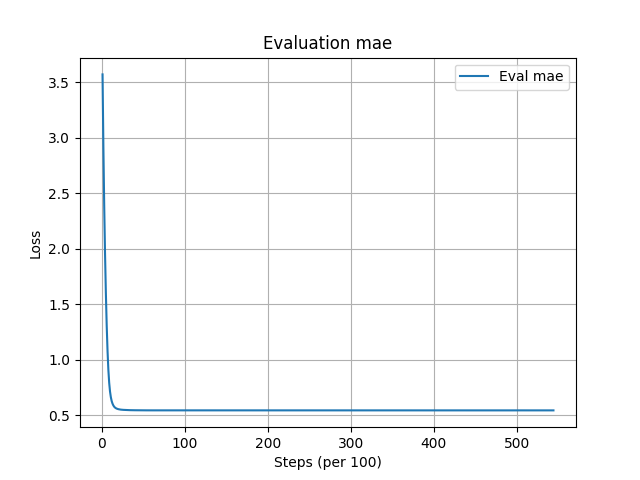
\includegraphics[width=\textwidth]{eval_loss_curve_re.png}  % 图片路径
    \caption{Evaluation Loss Curve(Regression)}
    \label{fig:eval_loss_curve_re}
\end{figure}
\begin{figure}[H]
    \centering
    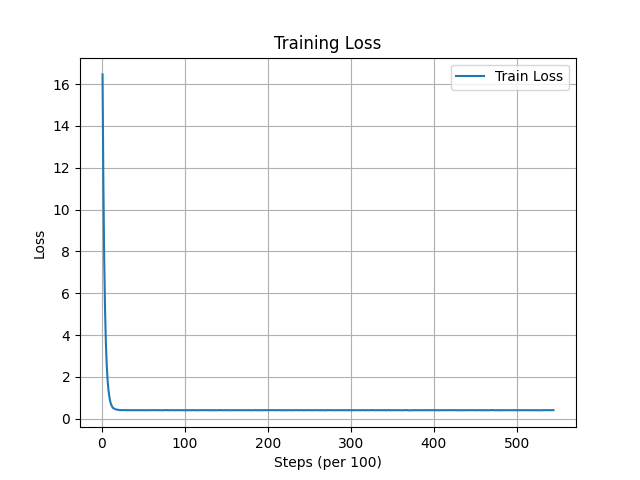
\includegraphics[width=\textwidth]{train_loss_curve_re.png}  % 图片路径
    \caption{Train Loss Curve(Regression)}
    \label{fig:train_loss_curve_re}
\end{figure}
\subsection{逻辑回归模型}
在表格中可以发现,最好结果为F1:0.79,AUC:0.83,在不同的学习率和batch size下随着轮数增多都能收敛到这一结果,说明对步长不敏感
\begin{figure}[H]
    \centering
    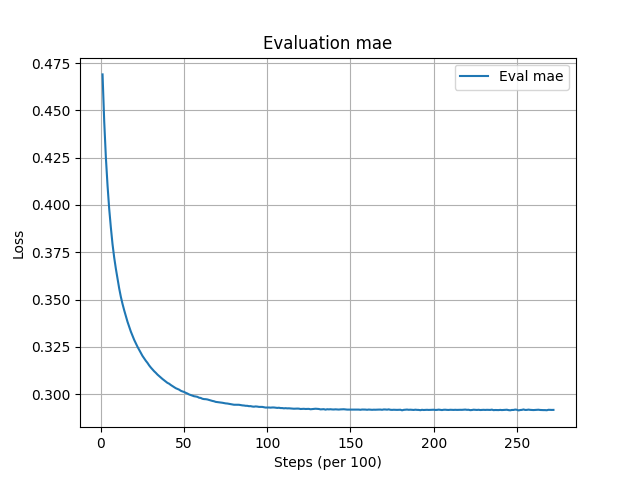
\includegraphics[width=\textwidth]{eval_loss_curve_cl.png}  % 图片路径
    \caption{Evaluation Loss Curve(classification)}
    \label{fig:eval_loss_curve_cl}
\end{figure}
\begin{figure}[H]
    \centering
    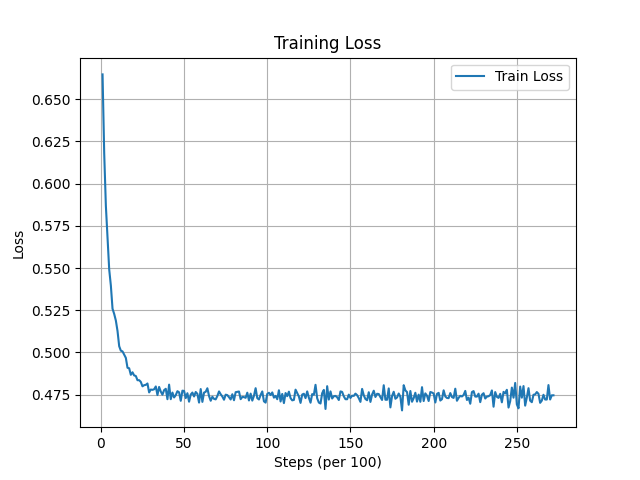
\includegraphics[width=\textwidth]{train_loss_curve_cl.png}  % 图片路径
    \caption{Train Loss Curve(classification)}
    \label{fig:train_loss_curve_cl}
\end{figure}

\section{课程反馈}

\subsection{花费的时间}
总计大概15h

\subsection{课程/实验建议}
希望能有更详细的实验细则(?)
其实现在已经很详细了

\end{document}
